\documentclass[]{article}
\usepackage{lmodern}
\usepackage{amssymb,amsmath}
\usepackage{ifxetex,ifluatex}
\usepackage{fixltx2e} % provides \textsubscript
\ifnum 0\ifxetex 1\fi\ifluatex 1\fi=0 % if pdftex
  \usepackage[T1]{fontenc}
  \usepackage[utf8]{inputenc}
\else % if luatex or xelatex
  \ifxetex
    \usepackage{mathspec}
    \usepackage{xltxtra,xunicode}
  \else
    \usepackage{fontspec}
  \fi
  \defaultfontfeatures{Mapping=tex-text,Scale=MatchLowercase}
  \newcommand{\euro}{€}
\fi
% use upquote if available, for straight quotes in verbatim environments
\IfFileExists{upquote.sty}{\usepackage{upquote}}{}
% use microtype if available
\IfFileExists{microtype.sty}{\usepackage{microtype}}{}
\usepackage{graphicx}
\makeatletter
\def\maxwidth{\ifdim\Gin@nat@width>\linewidth\linewidth\else\Gin@nat@width\fi}
\def\maxheight{\ifdim\Gin@nat@height>\textheight\textheight\else\Gin@nat@height\fi}
\makeatother
% Scale images if necessary, so that they will not overflow the page
% margins by default, and it is still possible to overwrite the defaults
% using explicit options in \includegraphics[width, height, ...]{}
\setkeys{Gin}{width=\maxwidth,height=\maxheight,keepaspectratio}
\ifxetex
  \usepackage[setpagesize=false, % page size defined by xetex
              unicode=false, % unicode breaks when used with xetex
              xetex]{hyperref}
\else
  \usepackage[unicode=true]{hyperref}
\fi
\hypersetup{breaklinks=true,
            bookmarks=true,
            pdfauthor={機械設計工程系二甲},
            pdftitle={2014 協同產品設計實習報告},
            colorlinks=true,
            citecolor=blue,
            urlcolor=blue,
            linkcolor=magenta,
            pdfborder={0 0 0}}
\urlstyle{same}  % don't use monospace font for urls
\setlength{\parindent}{0pt}
\setlength{\parskip}{6pt plus 2pt minus 1pt}
\setlength{\emergencystretch}{3em}  % prevent overfull lines
\setcounter{secnumdepth}{0}

\title{2014 協同產品設計實習報告}
\author{機械設計工程系二甲}
\date{April 30, 2014}

 
\usepackage{xeCJK}    % 中英文字行分開設置 
\usepackage[T1]{fontspec}    %設定字體用 
\usepackage{graphicx} 
\usepackage{fancyvrb} % for frame on Verbatim 
\usepackage{float}
\setCJKmainfont{新細明體}
\begin{document}
\maketitle

{
\hypersetup{linkcolor=black}
\setcounter{tocdepth}{3}
\tableofcontents
}
\section{協同產品設計實習期末報告(2ag7)}\label{ux5354ux540cux7522ux54c1ux8a2dux8a08ux5be6ux7fd2ux671fux672bux5831ux544a2ag7}

成員 49823207 40023207 40123110

\section{摘要}\label{ux6458ux8981}

本專案設計為利用網際網路達成協同產品設計之目的,使用者與設計者可以透過本專案進行設計溝通與創作。本專案利用git來進行版次管理、Creo來進行產品零件的設計與CMSimply來進行內容的管理,將零件儲存成STL格式上傳至CMSimply提供下載之功能,為了改善以往下載後需要該零件之繪圖軟體,才能看見該零件的不便,進而利用網路來展示零件之功能。
。

\section{緒論}\label{ux7dd2ux8ad6}

\begin{verbatim}
   在傳統上設計者在設計一項產品時,通常是由統籌者分配工作進行零件繪製、組合、分析等產品設計相關工作,但由於各專案組員零件版本的差異以及身處不同地域,而造成產品設計上的錯誤或是重疊性增高,使得設計時間增長,也增加了困難度令成本上升。
   為因應市場需求快速變化、產品生命週期縮短、全球化專業分工等趨勢,協同設計成為企業提升競爭力的方法之一。本專案主要探討協同設計過程中溝通產品品質與知識分享對於協同設計績效的影響;企業間因彼此需協同合作而建立夥伴關係,夥伴關係之良劣亦可能會對溝通品質與知識分享造成影響;而資訊科技能協助企業進行產品協同設計,其應用亦可能對合作夥伴間的溝通品質與知識分享發揮調節作用。
   產品協同設計的定義是在產品發展過程的所有相關人員,包括設計者、製造者、供應商、行銷人員等,都可同時參與產品開發並且互相溝通討論,即使身處不同地點的設計人員,也可透過網路同時進行某項產品的設計修改。   
   
\end{verbatim}

\section{文獻探討}\label{ux6587ux737bux63a2ux8a0e}

\subsection{一、協同設計的演進}\label{ux4e00ux5354ux540cux8a2dux8a08ux7684ux6f14ux9032}

協同設計(Collaborative Design)主要是由資訊運籌管理(Continuous
Acquisition and Life-cycle Support, CALS) 、同步工程(Concurrent
Engineering) 、 協同工程(Collaborative
Engineering)等相關的概念演進而來。

資訊運籌管理(CALS)的定義係指資訊整合、分享與交換;藉由作業程序的
改造、資料之資訊化及標準化,建立全球性共通商業系統以及無紙化作業環境,
將業務上所必要的資訊加以電子化、標準化,並運用資料庫系統和網路通訊系
統,使所有的資訊得以交換、共享為目標的策略。

CALS 最初是美國國防部所導入,主要是偏重在國防後勤支援,而目前企業
所引進的 CALS策略著重企業再造工程、整合資料庫支援產品生命週期、國際通
用標準(ISO)交換資料、及與Internet網路結合等觀念與技術的擴展。因此,產業
引進 CALS策略的目的在於再產品週期內創造一個整體數位資訊一元化的環
境,而產業相關上中下游的參與的協力廠商或客戶,可以藉由資訊的交換與資訊
的共享中獲得即時且必要的資訊,增進營運的效率與競爭力。

由於市場競爭的激烈,產品的多樣化與創新及快速的在市場銷售已成為企業
生存的必要條件。CALS在支援新產品的開發作業上之效益為縮短新產品的開發
與上市時間及降低產品開發過程中失敗的機率。CALS作業環境下,支援新產品
開發之方案包含以下: 1.
將產品意見透過Internet傳送到客戶手中,已結構化的方式蒐集客戶
意見,並直接傳送到客戶相關的資訊系統中,進行需求的彙整、分
析與評估,提供新產品開發與現有產品改良計劃之規劃。 2.
運用零件資料庫支援產品設計。 3. 運用電子圖檔交換同步進行。 4.
以產品資料管理系統(PDM)進行型態管理與設計流程管理。 5.
以電子會議進行設計審查作業。

同步工程(Concurrent Engineering)是一系統化的方法,有效地整合產品設
計以及相關程序,包括製造與其他的支援活動。此方法驅使設計者從設計初期即
考慮到整個產品生命週期所應該考慮的情形,包含品質、成本、排程與使用者需
求(Prasad, 1996)。

同步工程於新產品的開發過程是指製造部門人員早期涉入產品的開發過程,
其目的是為了消除研發與製造部門之間的衝突,改善研發與製造部門人員協調合
作的效率,提高新產品開發過程的效果。因此產品開發程序的整合或同步同程,
即是一種跨功能團隊的精神,例如;研發工程師和製造部門的工程師共事於同一
團隊,在這個團隊裏,研發工程師接收製造工程師的資訊輸入來配合設計,團隊
成員朝著共同目標邁進,團隊成員也都知道其他人在做什麼樣的工作,彼此相互
激勵前進,達成目標。

Carter and Baker(1992)指出在新產品開發過程中為了使設計、製造和生產三
者在新產品開發之初就有共同的認知,儘早發現設計上的盲點,提前檢討時間,
以減少日後在製造生產時發生問題的次數,進而降低開發成本,縮短產品開發時
間,以提昇產品品質及強化競爭力,因此在研發過程中所採用之同步工程,須具
備以下的基本理念: 1.
同步工程在新產品開發程序上是以彼此信任、共同分擔責任的多功
能團隊組織,著重的是客戶的預期反應。 2.
整合設計、製造與分析,以得到最佳化的產品與製程的設計方法 3.
系統化及同步化的同步工程開發環境。 4.
應用電腦技術使幾何圖形、知識庫與資料庫能充分結合溝通運用。

\subsection{二、協同設計的定義}\label{ux4e8cux5354ux540cux8a2dux8a08ux7684ux5b9aux7fa9}

協同設計(Collaborative Design)的定義為:「多位設計師在整個產品生命週期
中合作設計一個新產品的過程」(Shen, 2000)。 Kao and
Lin(1996)對協同設計作以下的定義,「一個協同設計系統必須提供
一個環境,讓身處兩個或更多不同地點的設計工程師,能夠藉由此系統,照平常
利用一般CAD的使用,達成協同的動作」。
因此,協同產品設計是「同步工程」概念的實現,讓涉及產品發展過程的所
有相關人員,包括設計者、製造者、供應商、行銷人員等,都可同時參與產品開
發並互相溝通討論,即使身處不同地點的設計人員,也可透過網路同時進行某項
產品的設計修改。其優點可使產品的開發成本降低、研發期縮短,同時提高使用
此類系統公司的競爭力。更重要的是,協同設計系統同時也能讓顧客參與產品設
計,研發出完全符合客制化的產品(盧永晟, 2001)。

\section{TeamProject}\label{teamproject}

本專案利用git來進行版次管理,解決各專案組員版次不一的情況,並記錄研究開發的過程;Creo可利用IE來進行更改產品零件相關參數的設定,進而可以讓客戶端進行零件的參數修改,以達成客製化之目的;再運用CMSimply來進行內容的管理,且將零件儲存成STL格式上傳至CMSimply提供下載之功能,讓專案組員可以利用網際網路隨時展示零件設計的進度,改善以往溝通不良的情形。
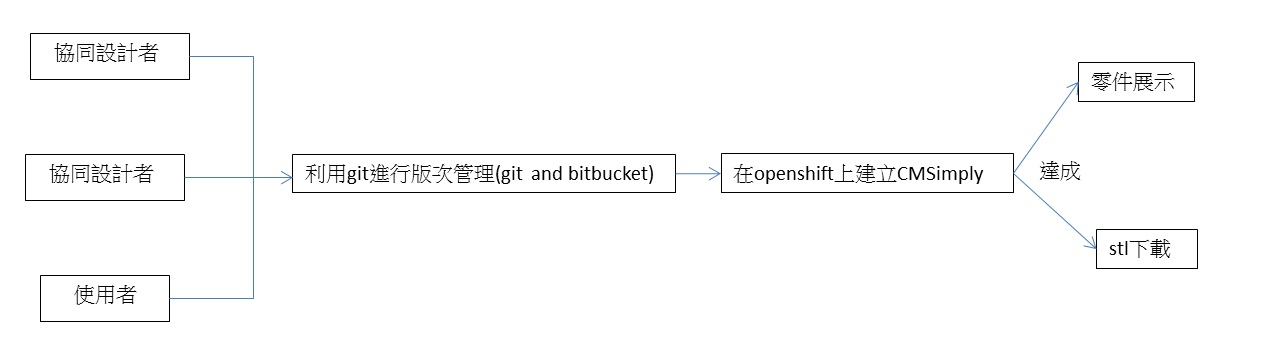
\includegraphics{./../images/2ag7/cdag7_01_process.jpg}

\begin{figure}[htbp]
\centering
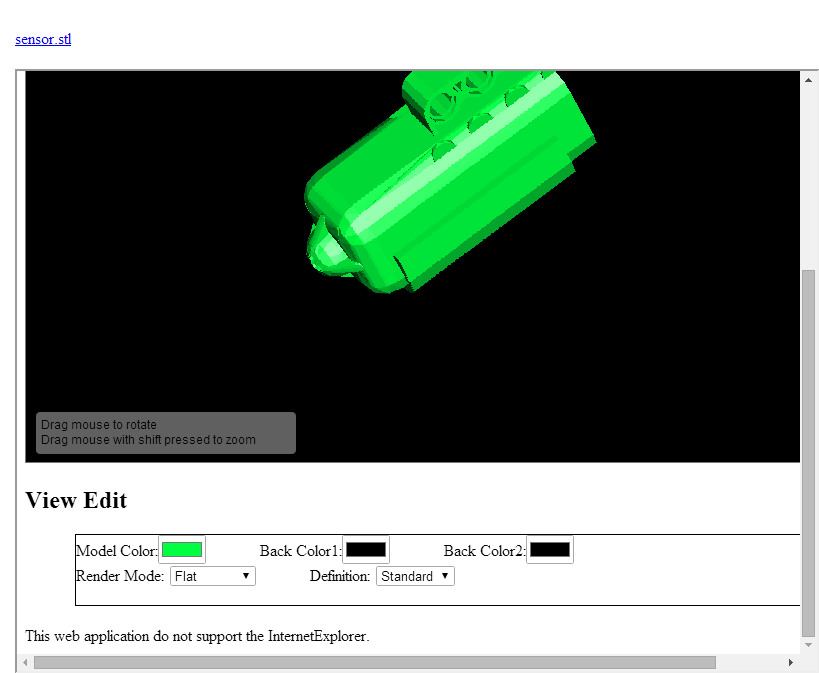
\includegraphics{./../images/2ag7/cdag7_02.png}
\caption{零件圖展示}
\end{figure}

\subsection{所需技術}\label{ux6240ux9700ux6280ux8853}

4.Creo 參數式零組件 2.Creo 自動零件組立程式 (Pro/Web.Link) 3.CherryPy
雲端程式 4.Python 3 資料庫查詢程式

\subsection{操作流程}\label{ux64cdux4f5cux6d41ux7a0b}

1.使用者準備好近端的 Creo 2.0 Pro/Web.Link 執行環境
2.使用者以嵌入式瀏覽器連結至雲端協同設計頁面
3.使用者根據所需的設計需求選擇設計表單
4.雲端程式根據使用者的選擇參數進行設計運算 5.使用者根據設計運算結果,
準備好近端的設計零件 6.使用者根據設計結果所提供的零件自動組立連結,
在近端完成所需的零件變更與自動組立

\section{結論}\label{ux7d50ux8ad6}

\begin{verbatim}
本次專案開發中,從零組件繪製到組立,利用雲端平台大幅縮短了專案時間;從手動到自動化組立,過程中更加了解以程式執行的快捷性和方便性,也減少因人為發生錯誤的機率。再用cherrypy寫出網頁架構利用leo add 整合資料進行管理,使用github進行版次的管理,利用openshfit的雲端平台與客戶端經驗分享和產品觀看交流,達成協同產品設計之目的。
在全球化競爭漸趨激烈的情況下,協同設計已經成為企業獲取與維持其競爭力的方法之一。希望未來能將此協同設計應用在企業而有所貢獻。對於實務上的
\end{verbatim}

意涵而言。除了重視資訊科技技術的的發展與應用之外,也應增進設計成員間之溝通能力,讓成員間能良好達到共同的理解設計情形。因此,企業將能增進協同設計的績效,如縮短研發週期時間與設計修改時間,使其增加其競爭力期能存活在競爭激烈的產業環境中。

\section{參考文獻}\label{ux53c3ux8003ux6587ux737b}

{[}1{]} http://pages.tzengyuxio.me/pandoc/

{[}2{]} http://wiki.mde.tw/doku.php

{[}3{]} Eynard, B., Lienard, S., Charles, S., \& Odinot, A. (2005).
Web-based collaborative engineering support system: Applications in
mechanical design and structural analysis. Concurrent
Engineering-Research and Applications, 13(2), 145-153.

{[}4{]} 劉佩芳(2005)。協同設計之驅動因素及對新產品開發績效之研究。亞洲
大學經營管理學系碩士班。

\end{document}
